\section{Calibration Campaigns}
\subsection{TPC Observables and PE Calibration}
For physics analysis in the TPC the following observables have to be calibrated\footnote{ToDo: Has PE already been introduced?} : 
\begin{itemize}
\item the scintillation signal S1, 
\item the ionization signal S2, 
\item the pulse shape discriminant F90, 
\item and the position information about a given event, namely the $t_{drift}$ variable, which encodes the event's Z-position and the XY-coordinates as is reconstructed from the relative fractions of S2 signal in the top PMT array \cite{DS50:first_paper}.
\item There are also derived variables such as the top-bottom asymmetry of S1, which are used in physics analyses, but need no independent calibration beyond the underlying variable.
\end{itemize}

Both S1 and S2 are calibrated in photo-electrons (PE), which is done in dedicated Laser calibration runs, in which the single PE charge spectra for each PMT are fitted and a PE-charge gain is determined. 

These Laser runs are also an integral part of a calibration campaign requiring a Laser run at least on each change in DAQ or CALIS configuration, such as drift field changes or source position changes.

\subsection{TPC Calibration with Internal Sources}
Prior to the insertion of external radioactive sources via CALIS the TPC could be calibrated using the $^{39}$Ar $\beta$-spectrum (end point 565 keV) and by injecting a $^{83m}$Kr into the Ar recirculation system\footnote{$^{83m}$Kr emits two conversion electrons at 32.1 keV and 9.1 keV, where the latter follows the former with a time constant of 154 ns \cite{Lippincott:83mKr}.}. These data sets have been used for a wide range of calibrations, including light yield, electron lifetime, position reconstruction, and tuning of the optics of the DarkSide-50 Geant-4 based Monte Carlo, called G4DS \cite{DS50:first_paper}. With the filling of the Underground Argon \cite{???}, $^{39}$Ar is not a dominant background anymore and can therefore not be used for calibration, instead gamma peaks from internal background, like $^{60}$Co originating in the cryostat, are being exploited to monitor the stability of the LY.

\begin{figure}[htbp]
 \centering
 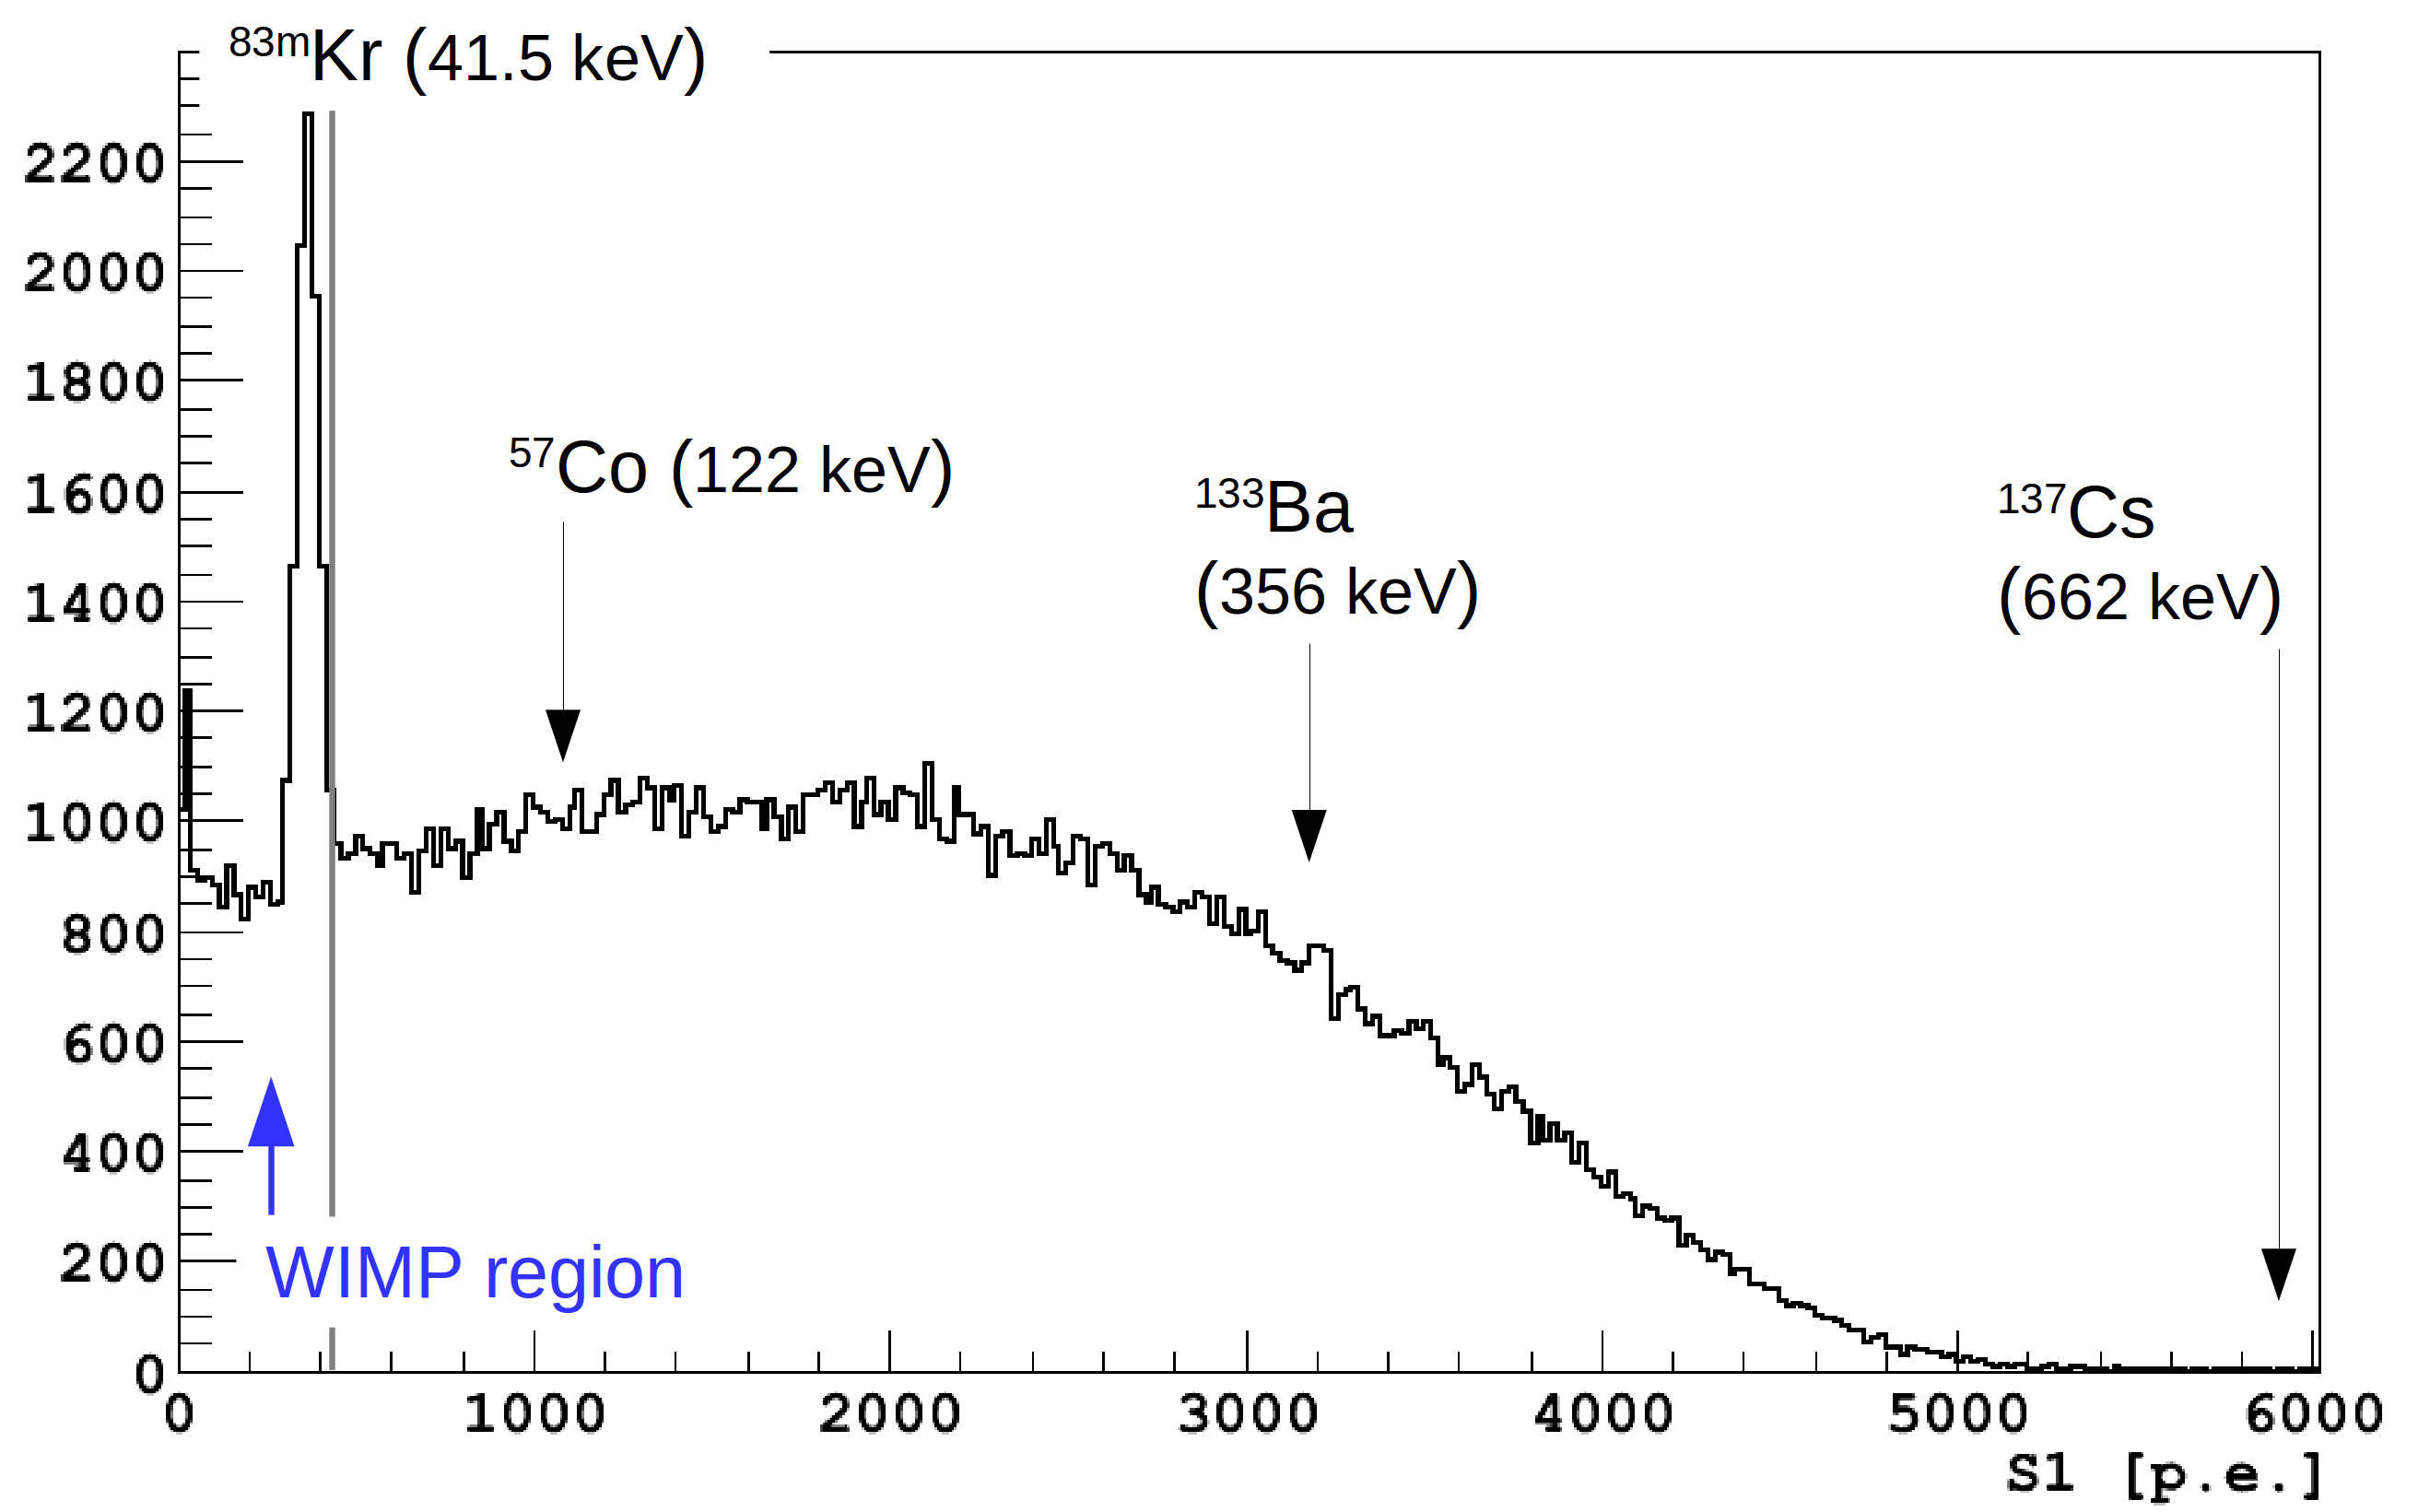
\includegraphics[width=0.8\textwidth]{Figures/GammaSources_Ar39spectrum.png}
 \caption{Scintillation spectrum (S1) at null field showing a $^{83m}$Kr peak on the $^{39}$Ar $\beta$ spectrum. The energies of the three gamma sources are indicated and cover the full range of the $^{39}$Ar spectrum.
\label{fig:GammaSources_Ar39spectrum}}
\end{figure}

\subsubsection*{DarkSide-50 Monte Carlo}
G4DS is a Geant-4 based ab-initio simulation of the energy deposits of each type of particle in LAr and in the materials building the detector, the generation of scintillation signals, and the light collection \cite{DS50:G4DS:paper}. Specific effort has been directed toward the accurate description of the materials and geometry of the entire detector (including the vetoes), the tuning of all the optical parameters affecting the photon propagation, and  the development of the LAr scintillation and ionization model. 
The poor experimental and theoretical constraints on electron-ion recombination in LAr obliged us to develop our own ad-hoc effective model. The functional form of the recombination probability was based on literature data, and parameter values were fit to make the full MC agree with the high statistics $^{39}$Ar spectrum measured in DarkSide-50. The overall photoelectron yield of the MC was normalized at the \ar\ endpoint. The entire Monte Carlo chain was then tested with the external calibration sources, $^{57}$Co, $^{133}$Ba and $^{137}$Cs. 


\subsection{Radioactive Sources}

For the calibration of the TPC's electron recoil (ER) response we selected $^{57}$Co, $^{133}$Ba and $^{137}$Cs to cross calibrate with the internal $^{39}$Ar, i.e.~cover the full $\beta$ spectrum (see Table \ref{tbl:GammaSources} and Fig.~\ref{fig:GammaSources_Ar39spectrum}). While all gamma sources enter the TPC active volume from outside, thanks to increasing interaction lengths as a function of energy the higher energy sources allow to cover larger fractions of the active volume. This allows to test the detector response (S1 and S2) as well XY reconstruction in different detector areas. 

\textit{this interaction length argument is a bit unclear, maybe even wrong! Bernd, June 24th}

%While gamma sources have the role of cross checking. They also allow to test detector response at edge regions of the detector, thereby acting as surface events. Which make data-MC discrepancies more pronounced in spectra, then they are for volume events.

For LSV calibration the gamma sources allow to study the LY as a function of energy in close proximity to the cryostat, which is a particularly critical detector region for neutron backgrounds originating in the TPC itself \cite{wright}. This can be cross checked with internal backgrounds: The C14 spectrum (beta spectrum with end point at ...) in the liquid scintillator of the LSV and $^{60}$Co originating in the cryostat steel (Sec.~\ref{sec:LSV:gammasources} and \cite{DS50:veto:paper}).

\begin{table}[htbp]
\caption{gamma sources}
\begin{tabular}{|l|l|l|l|l|}
\hline
\textbf{source} & \textbf{energy} & \textbf{half life} & \textbf{interact. length in LAr} & \textbf{activity}\footnote{as of October 2014} \\ \hline
$^{57}$Co & 122 keV & 0.744 y & 4.4 cm & 35 kBq \\ \hline
$^{133}$Ba & 356 keV & 10.54 y & 7.5 cm & 2 kBq \\ \hline
$^{137}$Cs & 662 keV & 30.2 y & 9.5 cm & 0.65 kBq \\ \hline
\end{tabular}
\label{tbl:GammaSources}
\end{table}

\subsubsection{Source Rate Optimization}
%\subsubsection{Source Selection}
After a preselection of gamma source energies, detailed studies with the DarkSide Monte Carlo G4DS were performed to select appropriate source activities and check the feasibility and physics reach of various deployment positions.

On the low activity end there is the necessity to gain sufficient statistics and a good signal/background ratio in the presence of nearly 50 Hz of trigger rate from $^{39}$Ar. On the high activity end the activity is constrainted by the requirement that event pile-up fraction is limited to a few percent, which is achieved by aiming at a source induced trigger rate of about 100 Bq in the TPC. Due to the different energies and different attenuation lengths of the various sources this results in significantly different source activity requirements. For $^{57}$Co ($^{137}$Cs) we used the source with the highest (lowest) activity available in the LNGS radioactive source repository \cite{LNGS:radioactivesourcelist}, while for the $^{133}$Ba all sources available at LNGS would have had a very high pile-up probability, instead a source with an activity of  1 $\mu$Ci at 1972 was procured from Temple radio safety \cite{Jeff:Ba133:privComm}.

Depending on different detector configurations, such as different drift field strengths, the DAQ can handle different trigger rates. Final adjustments of the source+$^{39}$Ar rate to a managable trigger rate were made by prescaling the whole energy spectrum.



\subsection{Neutron sources}
Unlike with $^{39}$Ar for ER there is by design very small neutron background which could be used for NR calibration, which is instead provided by the neutron source data, see Sec.~\ref{sec:CalibData:NR}). The analysis of neutron source data is heavily MC supported and so a realistic description of the detector components between the source and the active volume is an important factor when studying data-MC discrepancies. Here the gamma sources provide important input as well.

Two AmBe sources have been deployed, a high activity source with a nominal activity of 2000 neutrons/s and a low activity source (10 n/s). With the high activity source a high statistics sample of neutrons interacting in the TPC has been gathered, while with the low activity source TPC-LSV coincidences  and the study of the veto efficiency for nuclear recoils can be investigated. Due to PC only scintillator with a neutron capture time constant of $???$\footnote{DocDB ???}, this study was not possible with the high activity source due to event pile-up.



%different drift field changes
%with veto on and veto off.


\subsection{Timeline of the Calibration Campaigns}
Two calibration campaigns have been performed:
\begin{itemize}
\item The first extensive campaign involving all gamma sources and both the high and low activity AmBe neutron source took place in October and November 2014 at LNGS\footnote{has LNGS been introduced?}. The TPC was filled with atmospheric argon\footnote{has atmospheric argon been introduced and underground argon?} with an inherent trigger rate of nearly 50 Hz from $^{39}$Ar. The liquid scintillator of the LSV contained a PC only scintillator with $<0.1 \%$ TMB and 1.5 g/l PPO as wavelength shifter.
Fig.~\ref{???} shows the different configurations in which data has been taken as a function of source energy, source position and drift field.

\item In January and February 2015 a second campaign focusing on the LSV calibration using the low activity AmBe source was performed. Prior to that the LSV has been reconstituted with 5 \% TMB\footnote{what does 5 \% TMB mean? weight \%, volume \%?}. Two deployments were performed at two different PPO concentrations (0.7 g/l and 1.5 g/l), allowing to study the impact of the PPO concentration on alpha and gamma quenching. 1.5 g/l is our nominal PPO concentration.



\item All external radioactive source calibrations so far have been done with the TPC filled with atmospheric argon. An underground argon calibration campaign is planned for summer 2015 (Sec. \ref{sec:Outlook}).

%\item no mention of the collimator campaign, as this paper is already getting very dense.
\end{itemize}